\documentclass[12pt]{article}
%========宏包加载
\usepackage[a4paper,margin=2.5cm]{geometry}%设置页面格式,上下左右各留2.5cm
\usepackage[fancyhdr]{ctexcap} %中文
%\hypersetup{colorlinks=false}
\usepackage{amsmath,amssymb,amsthm} %公式
\usepackage{booktabs,longtable} %表
\usepackage{graphicx,float} %图
\usepackage{tikz}%绘图宏包
\usepackage{cite}%参考文献
\usepackage{setspace}%设定行距
\usepackage{lastpage} %记录最后一页的页码
\usepackage{wrapfig} %图文混排
\usepackage{titletoc} %
\usepackage{ccaption} %支持图表中英双标题
\usetikzlibrary{calc,intersections,through,backgrounds}%调用Tikz的libray

%========字体
\setCJKfamilyfont{huawen}{STXihei}
\setCJKfamilyfont{hwzhs}{STZhongsong}
\newcommand\xihei{\CJKfamily{huawen}}%华文细黑
\newcommand\zhongsong{\CJKfamily{hwzhs}}%华文中宋

%========标题格式
\CTEXsetup[format={\zihao{-4}\heiti\bf}]{section}%章节标题居左,四号,黑体
\CTEXsetup[format={\zihao{-4}\heiti\bf}]{subsection}%章节次标题居左,小四号,黑体
\CTEXsetup[format={\zihao{-4}\heiti\bf}]{subsubsection}
\newcommand\msection[1]{\section*{#1}\addcontentsline{toc}{section}{#1}}
%========页面格式
\pagestyle{fancy}
\renewcommand{\headrulewidth}{0pt}
\rhead{}\lhead{}
\fancyfoot[C]{\kaishu\small 第\thepage 页\quad 共~\pageref{LastPage} 页}


\linespread{1.5}%1.5倍行距
\setlength\lineskiplimit{0pt}\setlength\lineskip{1ex}%当间距太小时,跳一个ex

%========目录
\setcounter{tocdepth}{3}%目录深度设为3级
\newcommand\mycontents{\pagestyle{plain}\pagenumbering{Roman}\tableofcontents\newpage}
\renewcommand\contentsname{\centerline{\zihao{3} 目录}}

\makeatletter
\def\fnum@table#1{\tablename\nobreakspace\thetable\hspace{1em}}%去除表标题中的':'
\def\fnum@figure#1{\figurename\nobreakspace\thefigure\hspace{1em}}%去除图标题中的':'
\renewcommand*\l@section{\@dottedtocline{1}{0em}{1.0em}}
\makeatother
%========重定义命令
\def\emph#1{{\heiti #1}}

%========数学公式
\setlength\mathsurround{0.5ex}%文本公式前后留下空白
\makeatletter
\renewcommand\normalsize{\@setfontsize\normalsize\@xpt\@xiipt\abovedisplayskip8\p@\@plus3\p@\@minus5\p@\abovedisplayshortskip\z@\@plus3\p@\belowdisplayshortskip5\p@\@plus3\p@\@minus7\p@\belowdisplayskip\abovedisplayskip\let\@listi\@listI}%行间公式上下
\@addtoreset{equation}{section}
\renewcommand\theequation{\oldstylenums{\thesection}.\oldstylenums{\arabic{equation}}}%公式按章节编号
\makeatother

\allowdisplaybreaks %允许公式跨页

%========定理环境
\newtheoremstyle{mystyle}{5pt}{5pt}{\songti}{2em}{\heiti\bf}{}{1em}{}
%style名称 %环境前空白 %环境后空白 %主字体 %theorem名前的缩进 %theorem字体 % %theorem后缩进
\theoremstyle{mystyle}
\newtheorem{definition}{定义}[section]
\newtheorem{theorem}{定理}[section]
\newtheorem{corollary}{推论}[section]
\newtheorem{property}{问题}[section]
\newtheorem{proposition}{猜测}[section]
\newtheorem{lemma}{引理}[section]
\newtheorem{example}{例}[section]
\newenvironment{key}{\par\indent{\heiti 解~~}}{\hspace*{\fill} $\Box$\par}
\renewenvironment{proof}{\par\indent{\heiti 证明~~}}{\hspace*{\fill}$\Box$\par}

%========常用命令
\newcommand*\circled[1]{\hspace{1pt}\tikz[baseline=(char.base)]\node[very thin,shape=circle,draw,inner sep=.5pt,minimum size=2pt](char){#1};\hspace{1pt}}
\renewcommand\mod[1]{\ (\text{mod}\;#1)}
\newcommand{\upcite}[1]{$\!\!\!^{\mbox{\scriptsize\cite{#1}}}$}

%========论文封面
\def\maketitle{%
\begin{titlepage}\ttfamily
\begin{center}
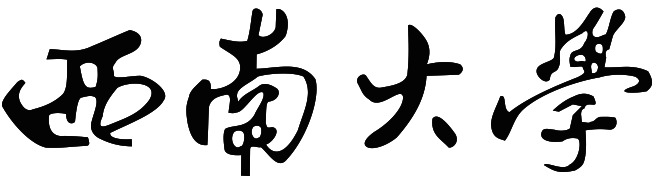
\includegraphics[width=2in]{swu.jpg}
\par\vspace{3em}
\zihao{1} {\heiti 本科毕业论文(设计)}
\vfil
\zhongsong\zihao{2} 题~~~~目\ \underline{\mbox{\title}}
\vfil
\begin{spacing}{2.0}%二倍行距
\zihao{-2}\ziju{.2}
\par\makebox[1.1in][s]{学院}~~\underline{\makebox[2.4in][c]{\college}}
\par\makebox[1.1in][s]{专业}~~\underline{\makebox[2.4in][c]{\major}}
\par\makebox[1.1in][s]{年级}~~\underline{\makebox[2.4in][c]{\grade}}
\par\makebox[1.1in][s]{学号}~~\underline{\makebox[2.4in][c]{\studentID}}
\par\makebox[1.1in][s]{姓名}~~\underline{\makebox[2.4in][c]{\author}}
\par\makebox[1.1in][s]{指导老师}~~\underline{\makebox[2.4in][c]{\don}}
\par\makebox[1.1in][s]{成绩}~~\underline{\makebox[2.4in][c]{}}
\end{spacing}
\vfil\zihao{3}\date\par\vspace{-4em}
\end{center}\end{titlepage}\newpage}

%========中文标题
\def\makezhtitle{%
\pagestyle{fancy}\setcounter{page}{1}\pagenumbering{arabic}
\begin{center}
    \heiti\zihao{3}\title\ 
    \par\hfill\par
    \zihao{-4}\songti \author\ 
    \par\zihao{5} 西南大学,重庆 400715
\end{center}
\par\hfill\par
}

%========英文标题
\def\makeentitle{%
\par\hfill\par
\begin{center}
    \zihao{4}\textbf{\entitle}
    \par\vspace*{1.7em}
    \zihao{5} \enauthor\ 
    \par\zihao{-5} School of Mathematics and Statistics, Southwest University, Chongqing  400715, China
\end{center}}

%========中文摘要
\newenvironment{abstrace}
{\maketitle\mycontents\makezhtitle\zhongsong\zihao{5} 摘要:\fangsong}
{\addcontentsline{toc}{section}{摘要}}
\def\keywords{\par\zhongsong 关键词:\songti}

%========英文摘要
\newenvironment{enabstrace}
{\addcontentsline{toc}{section}{Abstract}\makeentitle
\def\keywords{\par\noindent\textbf{Key words: }}
\par\vspace*{1.5em}\noindent\zihao{5}\textbf{Abstract:}}
{\par\pagebreak[4]\hspace{1em}}

\newenvironment{mybib}
{\begin{thebibliography}{99}
\setlength\itemsep{-2mm}\zihao{5}
\addcontentsline{toc}{section}{参考文献}}
{\end{thebibliography}}


\def\title{海伦三角形与海伦四面体}
\def\college{数学与统计学院}
\def\major{数学与应用数学}
\def\grade{2011级}
\def\studentID{222011314011208}
\def\author{王崇宁}
\def\don{王正攀}
\def\date{2015年5月21日}
\def\entitle{Heronian Triangle and Heronian Tetrahedron}
\def\enauthor{Wang Chongning}

\begin{document}
\zihao{-4}

\begin{abstrace}
对于海伦三角形, 本文给出一个研究工具, 也就是一个变换. 证明了这种变换可以简化海伦公式, 并保持海伦三角形的诸多性质. 然后在此基础上用更简单的方法证明了一些已有的结果. 本文还给出了几个用 Python 语言生成海伦三角形的程序. 在研究的过程中, 引入了二平方和以及佩尔方程的一些结论, 丰富了对海伦三角形的研究. 

对于海伦四面体, 本文给出了一些简单的性质. 发现了直角海伦四面体的存在性与完美长方体的存在性之间的关系. 重点论述了直角海伦四面体和等腰海伦四面体的一些性质. 
\keywords 海伦三角形; 海伦四面体; Python 语言
\end{abstrace}

\begin{enabstrace}
For Heronian triangles, in this paper, we give a research tool, which is a transformation. We prove that the transformation can simplify the Helen's formula, and preserve most properties of Heronian triangle. On the basis, we use simpler ways to prove some existing results. And several programs to make Heronian numbers are given in this paper. It is generated by the Python language. We also present some conclusions of quadratic sum and Pell's equation to enrich the study of Heronian  triangle.
\par\vspace*{.5em}\noindent
For Heronian tetrahedrons, some simple properties are given in this paper. We find the relation between the existence of isosceles Heronian tetrahedrons and perfect cuboids. Our focus is on the properties of right angle Heronian tetrahedrons and isosceles Heronian tetrahedrons.
\keywords Heronian triangle; Heronian tetrahedron; Python language
\end{enabstrace}%


\section{引言}
海伦三角形是一个有趣的话题, 寻找海伦三角形的性质和寻找特殊的海伦三角形一直为人们津津乐道. 古希腊数学家海伦提出了一个由三边长求三角形面积的公式, 由于这个公式如此之美, 后人研究边长和面积都是整数的三角形的时候,就把这种三角形称为海伦三角形. 

由于勾股三角形的两边长至少有一边是偶数, 所以勾股三角形全都是海伦三角. 另外, 维基百科的海伦三角形条目有一个定理说海伦三角形一定可以划分为两个直角三角形. 这说明海伦三角形和直角三角形的关系是紧密的. 本文将进一步挖掘这一层关系.

从三角形到四面体, 很容易想到有``海伦四面体''这样一个东西. 事实上, 确实有人研究过这样的四面体, 那就是边长都整数, 各个面的面积都整数, 体积也是整数的四面体. 这种四面体的存在就像是一个奇迹, 要找到一个都很困难. 本文将重点研究两种特殊的海伦四面体----直角海伦四面体和等腰海伦四面体. 

本文首先给出一个对研究海伦三角形非常有帮助的变换, 并证明这个变换的若干性质.

研究海伦三角形离不开海伦数组的生成, 相信前人已经做过这方面的研究, 但是没有详细的给出方法来, 本文将使用现今流行的 python 语言给出生成海伦三角形的程序.

对于海伦四面体, 国内的研究比较少, 本文类比海伦三角形给出一些简单的结果. 发现了直角海伦四面体的存在性和完美长方体的存在性是相关的, 因而直角海伦四面体的存在性还是一个很深的谜. 存在性虽然无法解决, 但是直角海伦四面体的性质还是可以研究的. 本文还研究了等腰海伦四面体, 并给出了一些简单的性质. 
\section{一些结果}
文\cite{daoxuan}中证明了一些本原海伦三角形的比较基本的性质: \par
(1)本原海伦三角形的三边长是两奇一偶.\par
(2)本原海伦三角形的最小边长是 3, 即不存在边长是 1 或 2 的本原海伦三角形.\par
(3)三原海伦三角形的面积$S$是 6 的倍数.\par
(4)三个连续自然数$2k-1,2k,2k+1$($k\ge2$为自然数)作为海伦三角形的三边长,当且仅当$k$是二阶递归数列$\{a_n\}$: $a_1=2$, $a_2=7$, $a_{n+2}=4a_{n+1}-a_n(n\ge1)$的项.\par

文\cite{denggao}给出等腰海伦数组的表示公式, 并对本原海伦三角形的两条边的公约数作了讨论: \par
(1)本原等腰海伦数组为$(s^2-t^2,s^2+t^2,2(s^2-t^2))$和$(s^2+t^2,s^2+t^2,4st)$其中$s,t$一奇一偶, $s\ge t$且$\gcd(s,t)=1$.\par
(2)对任意素数$p\equiv1\mod4$, 存在一个本原海伦数组中有二个数是$p$的倍数.\par
(3)对任意素数$p\equiv3\mod4$, 本原海伦数组中至多有一个数是$p$的倍数.\par
并提出一个问题, 海伦数组中三数能否都为平方数?

文\cite{huangxi}对这个问题作了回答, 给出了下述结果: 存在三边长均为平方数的本原等腰海伦三角形.

\section{一个线性变换}
现行海伦三角形的研究已有很多, 但是对于研究海伦三角形的工具的研究尚少, 所以本文首先给出一个工具, 并证明若干性质. 这个工具就是对三角形的三条边的一个变换, 在这个变换下海伦公式会变简单, 因而对海伦三角形性质的研究在一些帮助. 

海伦三角形是三边长和面积都是整数的三角形. 也有文献中称三边长及面积都为有理数的三角形为海伦三角形, 但这样的三角形必与某个整数型的海伦三角形相似, 所以本文不采用这个定义. 整数边长的直角三角形(即勾股三角形)都是海伦三角形, 这是因为勾股三角形必有一条偶数长的直角边. 锐角和钝角的海伦三角形也是大量存在的, 本文将用一种新的方法去研究海伦三角形的性质. 

设海伦三角形 $\triangle ABC$ 的三边长分别为 $a,b,c$, 令
    \begin{equation}\label{bianhuan}
         x=\frac{a+b-c}{2},\quad y=\frac{a+c-b}{2}, \quad z=\frac{b+c-a}{2}.
    \end{equation}

\begin{definition}
    如果整数 $a,b,c$ 可作为三角形的三边长, 且其面积为整数, 就说$a,b,c$可以构成\emph{海伦三角形}. 其中$a,b,c$就称之为\emph{海伦数}, 与之相应的 $x,y,x$ 称为\emph{海伦差数}. 
\end{definition}

下面将研究变换(\ref{bianhuan})的不变性, 以方便使用 $x,y,z$ 来研究海伦三角形. 

数学家海伦提出了以下公式: 
   \[S=\sqrt{p(p-a)(p-b)(p-c)}\quad (\text{其中} p=(a+b+c)/2). \]       

通过变换(\ref{bianhuan})容易得到
\begin{equation} \label{gongshi}
    S=\sqrt{(x+y+z)xyz}.        
\end{equation}

变换(\ref{bianhuan})一下子就把海伦公式简化了, 这将使得对海伦三角形的性质更容易被发现. 这个变换还保留的很多性质, 下面将分别介绍, 并给出证明. 因为变换中有分母, 所以要首先证明$x,y,z$是整数. 

\begin{theorem}\label{zhengshu}
    $x,y,z$ 是整数; 
\end{theorem}
\begin{proof}
    反设 $x=(a+b-c)/2$ 不是整数, 则 $a+b-c$ 是奇数. \par
    $a+b-c$ 是奇数蕴含 $a+c-b$ 是奇数, 否则就会引发 $2a=(a+b-c)+(a+c-b)$ 是奇数这个矛盾. 同理, 也蕴含 $b+c-a$ 是奇数. 于是 $a+b+c=(a+b-c)+(a+c-b)+(b+c-a)$ 也是奇数. \par
    所以\[\bigg(\frac{a+b+c}{2}\bigg) \bigg(\frac{a+b-c}{2}\bigg) \bigg(\frac{a+c-b}{2}\bigg) \bigg(\frac{b+c-a}{2}\bigg) = S^2\]
    不是一个整数, 这与面积 $S$ 是一个整数相矛盾. 
\end{proof}

从证明中我们看到$a+b-c$是一个偶数, 这对$a,b,c$的奇偶性有什么影响呢?下面来分析一下. 如果全是偶数, 没有任何矛盾; 如果有两个偶数一个奇数, 那么$a+b-c$是奇数, 这是不可能的; 如果有一个偶数, 两个奇数, 那么$a+b-c$是一个偶数; 如果全是奇数, 那么$a+b-c$是一个奇数, 这也是不可能的. 综上所述, 可得如下推论:

\begin{corollary}
$a,b,c$要么全是偶数, 要么是两奇一偶. 
\end{corollary}

在定理\ref{zhengshu} 的证明中, 有$a+b+c$是偶数这个结果, 于是有

\begin{corollary}
海伦三角形的周长必是偶数. 
\end{corollary}

证明了$x,y,z$是整数, 然后自然要考虑变换(\ref{bianhuan})是不是可逆的. 既然$a,b,c$可以唯一确定一组$x,y,z$, 那么反过来给定一组$x,y,z$的话, 能不能唯一确定一组$a,b,c$呢?答案是肯定的. 
   
\begin{theorem}
    变换\rm(\ref{bianhuan})是可逆的, 即 $x,y,z$ 和 $a,b,c$ 是相互唯一确定的. 
\end{theorem}
    
\begin{proof}
    由变换(\ref{bianhuan})可以反解出
    \begin{equation}\label{nibianhuan}
        a=x+y, \quad b=x+z, \quad c=y+z.
    \end{equation}
即得所证. 
\end{proof}

这样一来, 每求出一组满足条件的$x,y,z$就可以得到一组相应的海伦数$a,b,c$. 由于使用$x,y,z$可以使海伦公式变得简单, 因此, 我们可以通过研究$x,y,z$的性质来研究海伦三角形, 从而简化证明过程. 现在我们要证明变换(\ref{bianhuan})可以保持海伦三角形的诸多性质. 

有的海伦三角形相似于其他比它更小的海伦三角形, 有的海伦三角形则不相似于比它更小的海伦三角形. 后者我们称为本原海伦三角形, 因为通过把本原海伦三角形扩大我们可以得到所有的海伦三角形. 后面会单独研究本原海伦三角形, 下面证明的定理为我们提供一个通过$x,y,z$判定一个三角形是不是本原海伦三角形. 

海伦三角形是本原的当且仅当$a,b,c$的最大公约数是 1. 因此下面的定理将非常有用. 
    
\begin{theorem}
    $\gcd(a,b,c)=\gcd(x,y,z)$; 
\end{theorem}
\begin{proof}
    设 $\gcd(a,b,c)=m$, 令 $a=a_1m,\ b=b_1m,\ c=c_1m$, 则 $\gcd(a_1,b_1,c_1)=1$. 我们有
    \begin{equation}
        x=m\frac{a_1+b_1-c_1}{2}=mx_1,\ y=m\frac{a_1+c_1-b_1}{2}=my_1,\ z=m\frac{b_1+c_1-a_1}{2}=mz_1
    \end{equation}
    设 $\gcd(x_1,y_1,z_1)=n$, 由 $a_1=x_1+y_1$ 知 $n|a_1$, 同理 $n|b_1,\ n|c_1$, 所以 $n=1$. \par
    这就证明了 $\gcd(a,b,c)=m=\gcd(x,y,z)$.
\end{proof}

当$x,y,z$的最大公约数为$1$的时候, $a,b,c$就可以构成本原海伦三角形. 同理当$x,y,z$的最大公约数不为$1$的时候, $a,b,c$就构不成本原海伦三角形. 
    
三个正整数$a,b,c$可以构成海伦三角形的必要条件是$a,b,c$可以构成三角形, 在$a\le b\le c$的前题下, 就变成$a,b,c$构成本原海伦三角形等价于$a+b>c$. 那么$x,y,z$可以通过变换构成三角形的充要条件是什么呢?或许答案比较简单, 如果这样, 就说明变换(\ref{bianhuan})是优良的. 

\begin{theorem}
    正整数$a,b,c$ 可以构成三角形的充要条件是 $x,y,z$ 都是正整数; 
\end{theorem}
\begin{proof}
    (必要性)若正整数$a,b,c$ 可以构成三角形, 则
     \[a+b-c>0, \quad a+c-b>0, \quad b+c-a>0. \]
     由定理(\ref{zhengshu})及变换式(\ref{bianhuan})
可知 $x,y,z$ 都是正整数. \par
    (充分性)由逆变换(\ref{nibianhuan}), $a+b-c=x+y+x+z-y-z=2x>0$,同理可得$a+c-b>0$, 以及$b+c-a>0$, 所以这样得到的$a,b,c$可以构成三角形. 
\end{proof}

在证明的过程中, 我们可能会发现很多情况下假定$a\le b\le c$有利于简化证明. 于是会想到, $a,b,c$的大小关系反映在$x,y,z$上成是怎么样的呢?不难发现下述定理. 
\begin{theorem}
    $a\le b\le c\iff x\le y\le z. $
\end{theorem}

\begin{proof}
    证明很简单, 此处从略. 
\end{proof}

上面这个公式中我们用了小于等于号, 其实, 两个不等号是不可能同时取到的. 因为当$a=b=c$时, $S=\sqrt3a^2/4$, 这种情况下面积始终是一个无理数. 这说明海伦三角形不可能是等边三角形. 两个不等号不能同时取到, 退而求其次, 一个不等号能不能取到呢?答案是肯定的, 后面会单独研究一个等号取到的情形------ 等腰海伦三角形. 现在我们要回答的是当$a\le b\le c$中取到一个等号时, $x\le y\le z$是不是也同样取到一个等号, 取到等号的位置是不是相同?

\begin{theorem}
    $\bigtriangleup ABC$ 等腰当且仅当 $x=y$ 或 $y=z$. 
\end{theorem}
\begin{proof}根据式(\ref{nibianhuan})
    \begin{align*}
        a & =b\iff x+y=x+z\iff y=z ; \\
        b & =c\iff x+z=y+z\iff x=y . 
    \end{align*}
\end{proof}

既然海伦三角形的三边长不可能全部相等, 我们就要提问, 海伦三角形的三边长能不能构成一个等差数列, 更特殊的, 海伦三角形能不能由三个连续的正整数构成它的边长?答案是肯定的, 后面我们将单独研究这种三角形, 现在我们先回答这种三角形怎样由$x,y,z$刻画?
    
\begin{theorem}
    $a,b,c$ 是等差数列当且仅当 $x,y,z$ 是等差数列. 特别地 $a,b,c$ 是连续正整数当且仅当 $x,y,z$ 是连续正整数. 
\end{theorem}
\begin{proof}
    \[2b=a+c\iff2(x+z)=(x+y)+(y+z)\iff 2y=x+z, \]
    这说明二者成等差数列是等价的. \par
    \[b-a=(x+z)-(x+y)=z-y, c-b=(y+z)-(x+z)=y-x, \]
    这说明成等差数列时二者的公差是相等的. 
\end{proof}

准备好了用海伦差数$x,y,z$来研究海伦三角形的性质, 后面我们会用它们来证明一些海伦三角形的一些性质. 

\section{生成海伦数}
\subsection{用 Python 生成海伦数}
讨论了这么多关于海伦三角形的知识, 读者可能早就想看到一些海伦三角形. 假如根本没有海伦三角形, 或者只有很少的海伦三角形, 我们的研究又有什么意义呢?所以, 现在我们使用编程的方法来生成海伦三角形. 
    
研究海伦三角形最好的方法是从已知的海伦三角形出发, 这就需要我们知道已知的海伦三角形有哪些. 

下面的程序将使用 Python 语言, 因为这门语言相对于 C 语言来说比较高级, 容易读懂; 而且 Python 的库中有大量的数学工具, 它们大多在 C 语言级别实现, 速度也快, 调用又非常方便, 所以用 Python 来研究再好不过. 我们会用到 Python 的 Numpy 和 gmpy2 模块. 

给定周长$n$的时候, 我们采用遍历$a,b,c\ (\text{其中}\ a+b+c=n)$的方法来找到海伦三角形. 首先要判断$a,b,c$是否构成一个海伦三角形, 然后判断它的面积是不是一个整数. 我们发现第一步在遍历的时候就可以完成. 首先假定$a\le b\le c$且等号不同时成立. 这样有$1\le a\le n/3$, 确定了$a$的范围, 我们再来确定$b$的范围, 由于$a\le b\le c$且$a+b>c$且$a+b+c=n$, 消去$c$得到$n/2-a<b\le(n-a)/2$且$a\le b$即$\max=(2a,n-2a+1)\le2b\le n-a$, 最后$c$的取值就被定了下来$c=n-a-b$. 

下面的程序将按周长从小到大依次输出可以构成三角形的三边长, 当然都是整数. 
\begin{verbatim}
    for n in range(3,100):
        a=1
        while a<n/3:
            b=max(a,n//2-a+1)
            while b<=(n-a)//2:
                c=n-a-b
                print([a,b,c])
                b+=1
            a+=1    
\end{verbatim}

这里是从周长为 3 开始的, 但实际上通过计算, 边长最小的海伦三角形的边长是 12. 另外, 由于海伦三角形周长一定是偶数, 所以$n$只需遍历大于等于 12 的偶数就可以了. 又$p=n/2$, 只需要让$p$遍历大于等于 6 的整数就行了. 而且从$a=1$开始也没有必要, 请看下面的定理. 

\begin{theorem}
    有一条边长为 $1$ 或 $2$ 的海伦三角形不存在, 有一条边长为 $3$ 的海伦三角形有无限多个. 
\end{theorem}
\begin{proof}
    假定 $a\le b\le c$, $a=1$ 意味着 $x=0$, 这是不可能的. $a=2$ 意味着 $x=y=1$, $S^2=z(z+2)$, 这与 $z(z+2)$ 不能是完全平方数矛盾. 所以海伦三角形的边长至少为 3. \par
    不难验证当 $x=1,\ y=2,\ z=a_n,\ a_n=6(a_{n-1}+1)-a_{n-2},\ a_0=0,\ a_1=3$ 时, 可得有一条边长为 3 的海伦三角形, 所以此类海伦三角形有无限多个. 
\end{proof}

在海伦公式$S=\sqrt{p(p-a)(p-b)(p-c)}$中, 由于海伦三角形的周长$a+b+c$是偶数, 所以$p,\ p-a,\ p-b,\ p-c$都是整数, 所以判断面积是不是整数, 只需要判断$p(p-a)(p-b)(p-c)$是不是完全平方数. 如下Python程序将依次生成海伦三角形
\begin{verbatim}
    from gmpy2 import is_square
    for p in range(6,1000):
        a=3
        while a<2*p/3:
            b=max(a,p-a+1)
            while b<=(2*p-a)//2:
                c=2*p-a-b
                s=p*(p-a)*(p-b)*(p-c)
                if gp.is_square(s):print([a,b,c])
                b+=1
            a+=1
\end{verbatim}

既然我们有$x,y,z$, 构成三角形只要它们都是正数就可以了, 为什么不用$x,y,z$来生成海伦三角形呢?
\begin{verbatim}
    from gmpy2 import is_square
    n=30
    for x in range(1,n//3+1):
        for y in range(x,(n-x)//2+1):
            for z in range(y,n+1):
                if gp.is_square(x*y*z*(x+y+z)):print([x+y,x+z,y+z])
\end{verbatim}



\subsection{从已有的海伦数生成新的海伦数}
从已有的海伦数生成海伦数的最简单的方法就是乘以一个正整数$k$, 所得海伦数的周长扩大$k$倍, 面积扩大$k^2$倍. 
   
\begin{theorem}
    若$(a,b,c)$为海伦数, 则$(ka,kb,kc),k=1,2,3,\cdots$也是海伦三角形. \end{theorem}

勾股数都是海伦数, 用勾股数很容易得到海伦数. 

\begin{theorem}
    设两组勾股弦数组中有一直角边相同, 即有$(a,b_1,c_1)$和$(a,b_2,c_2)$, 则数组$(b_1+b_2,c_1,c_2)$和$(b_1-b_2,c_1,c_2)$均为海伦数. 
\end{theorem}
\begin{proof}
如图, 根据已知条件, 两个直角三角形可以组成一个大三角形, 或者从在三角形中减去小的, 得到一个小三角形, 无论哪种情况, 都得到一个新的海伦三角形. \par
    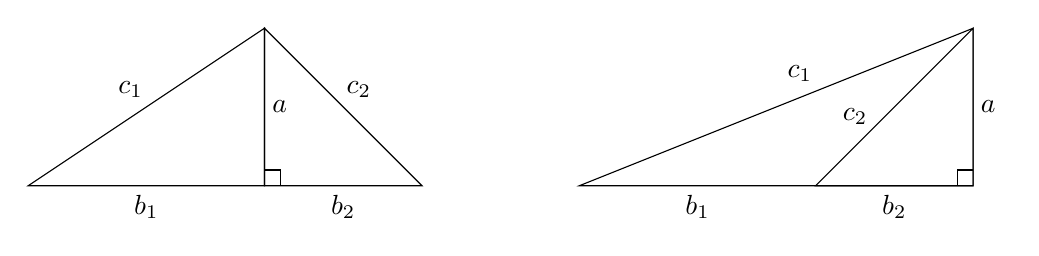
\begin{tikzpicture}
	\draw(0,0)--(3,2)--(3,0)--cycle;
	\draw(5,0)--(3,2)--(3,0)--cycle;
	\draw(3,.2)--(3.2,.2)--(3.2,0);
	\node[right]at(2.9,1){$a$};
	\node[below]at(1.5,0){$b_1$};
	\node[below]at(4,0){$b_2$};
	\node[above]at(1.3,1){$c_1$};
	\node[above]at(4.2,1){$c_2$};
	\draw(7,0)--(12,2)--(12,0)--cycle;
	\draw(10,0)--(12,2)--(12,0)--cycle;
	\draw(11.8,0)--(11.8,.2)--(12,.2);	
	\node[right]at(11.9,1){$a$};
	\node[below]at(8.5,0){$b_1$};
	\node[below]at(11,0){$b_2$};
	\node[above]at(9.8,1.2){$c_1$};
	\node[above]at(10.5,.65){$c_2$};
    \end{tikzpicture}
\end{proof}

\begin{corollary}\label{shengchengerbei}
    任取一组勾股弦数组$(x,y,z)(x\ne y)$, 则$(2x,z,z),(2y,z,z)$都是海伦数, 且对应的海伦三角形面积相等. 
\end{corollary}

从一个勾股三角形, 可以得到两个等腰海伦三角形, 于是问题来了:是否所有的等腰海伦三角形都可以以这种方式由勾股三角形生成?本文将在“等腰海伦三角形”一节中回答这一问题. 
\begin{theorem}
设$(a_1,b_1,c_1)$和$(a_2,b_2,c_2)$为两组勾股弦数组, 则以下$8$组数组均为海伦数\upcite{jianyi}. 
\begin{align*}
&(a_1a_2+b_1b_2,a_1c_2,b_2c_1);\ (|a_1a_2-b_1b_2|,a_1c_2,b_2c_1);\\
&(a_1a_2+b_1b_2,b_1c_2,a_2c_1);\ (|a_1a_2-b_1b_2|,b_1c_2,a_2c_1);\\
&(a_1b_2+a_2b_1,a_1c_2,a_2c_1);\ (|a_1b_2+a_2b_1|,a_1c_2,a_2c_1);\\
&(a_1b_2+a_2b_1,b_1c_2,b_2c_1);\ (|a_1b_2+a_2b_1|,b_1c_2,b_2c_1).
\end{align*}
\end{theorem}



\section{海伦三角形的性质}
海伦三角形是一种特殊的三角形, 当然具有一般的三角形所不具有的性质, 下面将主要考察本原海伦三角形的性质. 前面已经提到过本原海伦三角形, 其实研究海伦三角形, 只要把本原海伦三角形研究清楚就可以了. 接下来研究等腰海伦三角形、等差海伦三角形、面积与边长相等的特殊的海伦三角形等等. 

本节定理有些是已经写过的, 由于本文引入了一个变换, 可以将证明简化不少, 所以重新证明一下. 

\subsection{本原海伦三角形}
\begin{definition}
     如果 $\gcd(a,b,c)=1$, 就称海伦 $\triangle ABC$ 是\emph{本原海伦三角形}
\end{definition}

\begin{theorem}\label{erji}
    本原海伦三角形的三边长必定是二奇一偶\upcite{daoxuan}. 
\end{theorem}
\begin{proof}
    这个定理前面实际上证明过, 当时使用的是$(a+b-c)/2$是一个整数这一事实. 下面我们再用另外一种方法证明一下. \par
    因为 $\gcd(x,y,z)=\gcd(a,b,c)=1$, 所以 $x,y,z$ 不能全是偶数. 又因为 $a=x+y,b=x+z,c=y+z$, 所以 $x,y,z$ 不能全是奇数. 因此 $x,y,z$ 中恰有一个奇数或恰有两个奇数, 无论是哪种情况, 都将导致 $a,b,c$ 中二奇一偶. 
\end{proof}

\begin{corollary}
    海伦三角形的三边长要么全是偶数, 要么二奇一偶. 
\end{corollary}

这个推论如此之简单, 而且看起来没有什么用处, 其实不然, 我们后面将会用这个推论证明一些事情. 所以一些伟大的发现往往都有一个简单和出发点, 但是由此延伸出去的知识, 可能会令你大加赞叹. 
    
\begin{theorem}\label{mianji6}
    本原海伦三角形的面积$S$是 6 的倍数\upcite{daoxuan}. 
\end{theorem}
\begin{proof}
     不妨设$\triangle ABC$ 是本原的, 仅需证 2 和 3 都整除 $(x+y+z)xyz$. \par
     首先, 由定理(\ref{erji})的证明过程可知 $x,y,z$ 中必有一个偶数, 故 $2|(x+y+z)xyz$. \par
     其次, 由同余理论可知完全平方数不可能模 3 余$-1$, 所以
     \[(x+y+z)xyz=S^2\not\equiv1\mod3. \]
     若 3 整除 $x,y,z$ 中的一个, 结论已明. 否则, 若 $x,y,z$ 模 3 的最小剩余分别是 1,1,1 或 -1,-1,-1, 则 $3|(x+y+z)$, 结论亦真. 再不然, 最小剩余分别是 -1,1,1 的话, 与 $(x+y+z)xyz\not\equiv1\quad\mod3$ 矛盾, 其它情况同理可以排除. 因此 $3|(x+y+z)xyz$.
\end{proof}

\begin{corollary}\label{gougu3}
    勾股三角形至少有一条直角边是 3 的倍数. 
\end{corollary}
\begin{proof}
    设勾股三角形的三边长分别为$a,b,c$, 其中$a,b$为直角边, 则面积
    \[S=ab/2.\]
    由$6|S$, 得$3|S$, 因而$3|ab$, 所以$3|a$或$3|b$.
\end{proof}

\begin{theorem}
    本原海伦三角形任意两边的公因子模 $4$ 余 $1$\upcite{denggao}. 
\end{theorem}
\begin{proof}
    \circled1设$q$是素数, 且$q\equiv3\mod4$.\par
    令$p=(a+b+c)/2$, 则本原海伦三角形的面积的平方为
    \begin{align*}
        S^2&=p(p-a)(p-b)(p-c)\\
        &=p(p^3-(a+b+c)p^2+(ab+ac+bc)p-abc)\\
        &=p[-p^3+(ab+ac+bc)p-abc]
    \end{align*}
    若$q$是$a,b$的公因子, 则
    \[s^2\equiv-p^4\mod q\]
    这说明(这里$\binom ap$是 Jacobi 符号)
    \[\dbinom{-p^4}{q}=1, \]
    另一方面, 由于$q\equiv3\mod4$, 所以
    \[\dbinom{-p^4}{q}=\dbinom{-1}{q}\dbinom{p^4}{q}=\dbinom{-1}{q}=-1,\]
    互相矛盾, 所以本原海伦三角形的任意两边的公因子不能有模 4 余 3 的素数. \par
    \circled2由于本原海伦三角形的三边长两奇一偶, 所以它的任意两边的公因子不是 2 的倍数. \par
    综合\circled1\circled2, 若$m$是本原海伦三角形两边的公因子, 不妨设
     \[m=p_1p_2\cdots p_k\ (p_i\text{是素数}),\]
    则$p_i\equiv1\mod4$, 故$m\equiv1\mod4$.
    这就证明了这个定理. 
\end{proof}

\begin{corollary}
    本原海伦三角形至多有一条边被 3 整除. 
\end{corollary}

    
\subsection{等腰海伦三角形}
\begin{lemma}
    设正整数 $m,n$ 互素, $mn$ 是完全平方数的充要条件是 $m$ 和 $n$ 都是完全平方数\upcite{cihe}. 
\end{lemma}
\begin{proof}
    若 $m=1$ 或 $n=1$, 结论显然. 下面假定 $m,n>1$.\par
    设 $m,n$ 的标准分解式分别为
    \begin{align*}
        m &= p_1^{\alpha_1}p_2^{\alpha_2}\cdots p_s^{\alpha_s} \\
        n &= q_1^{\beta_1}q_2^{\beta_2}\cdots q_t^{\beta_t}
    \end{align*}
    由于 $m,n$ 互素, 以故 $p_i$ 与 $q_i$ 互不相同. 又 $mn$ 是完全平方数, $\alpha_i, \beta_i$ 都是偶数. 所以 $m,n$ 都是完全平方数. 
\end{proof}

\begin{theorem}
    本原等腰海伦三角形 $a,a,b$ 所确定的 $x,x,z$ 一定可以由下式得出, 而且下式必定给出海伦三角形:
    \begin{equation}\label{dengyao1}
        \begin{cases}
            z=2m^2\\
            x=y=n^2-m^2
        \end{cases}
        \quad m,n\in N^+ \text{且} m<n
    \end{equation}
    \begin{equation}\label{dengyao2}
         \hspace{3.2em}\begin{cases}
              z=(2m+1)^2\\
              x=y=[(2n+1)^2-z]/2
         \end{cases}m,n\  \text{是奇数且} m<n
    \end{equation}
\end{theorem}
\begin{proof}
    首先证明可构成海伦三角形. 对于 (\ref{dengyao1}) 式
    \[(x+y+z)xyz=[2(n^2-m^2)+2m^2](n^2-m^2)^22m^2=[2mn(n^2-m^2)]^2\]
    对于 (\ref{dengyao2}) 式
    \[(x+y+z)xyz=n^2{\bigg(\frac{n^2-m^2}{2}\bigg)}^2 m^2\]
    都是完全平方数, 即得所证. \par
    下面证明本原等腰海伦三角形可由(\ref{dengyao1})或(\ref{dengyao2})表出. \par
    设$\bigtriangleup ABC$ 是本原等腰海伦三角形, 不妨设 $x=y$, 有 $\gcd(x,z)=1$, 由 $S^2=(2x+z)x^2z$ 是完全平方数得 $z(2x+z)$ 是完全平方数. \par
    (i)若 $z$ 是偶数, 设 $z=2k$, 因为 $z(2x+z)=2^2k(x+k)$, 所以 $k(x+k)$ 是完全平方数. 又 $\gcd(x,x+k)=\gcd(x,k)\le\gcd(x,z)=1,\ \gcd(x,x+k)=1$, 由引理, $k,x+k$ 都是完全平方数. 设 $z=2m^2,\ x+m^2=n^2$, 立得 $x,y,z$ 可由 (\ref{dengyao1}) 式表出. \par
    (ii)若 $z$ 是奇数, 同理, $z$ 和 $2x+z$ 都是完全平方数. 设 $z=m^2$, $2x+z=n^2$, 立得 $x,y,z$ 可由 (\ref{dengyao2}) 式表出. 
\end{proof}

\begin{corollary}\label{dengyao}
     本原等腰海伦三角形 $a,a,b$ 一定可以由下式得出, 而且下式必定给出等腰海伦三角形:
     \begin{equation}\label{dengyaoyi}
         \begin{cases}
              a=b=n^2+m^2\\
              c=2(n^2-m^2)
         \end{cases}
         m,n\in N^+ \text{且} m<n
     \end{equation}
     \begin{equation}\label{dengyaoer}
          \hspace{2.3em}\begin{cases}
               a=b=(n^2+m^2)/2\\
               c=n^2-m^2
          \end{cases}m,n\  \text{是奇数且} m<n
     \end{equation}
\end{corollary}

下面我们将用到一些二平方和的知识\upcite{keqin}. 一个正整数能表示能两正整数的平方和, 就称这个数是二平方和. 欧拉证明了如下定理:素数 $p$ 是二平方和的充要条件是 $p=2$ 或 $p\equiv1\mod4$. 高斯证明了如下定理(高斯定理):正整数 $n$ 是二平方和的充要条件是 $n$ 的无平方因子部分 $m'$ 或者为 $1$, 或者 $m'$ 的每个素因子均是二平方和(这意味着 $m'$ 的每个素因子均为 $2$ 或模 $4$ 余 $1$ 的数).  

\begin{theorem}
     本原等腰海伦三角形必成对出现, 即若 $a,a,c$ 能构成, 则存在 $c'\neq c$ 使 $a,a,c'$ 也能构成. 
\end{theorem}
\begin{proof}
     由于本原海伦三角形三边长二奇一偶, 因此 $a$ 必为奇数. 由高斯定理, $a$ 是二平方数当且仅当 $2a$ 是二平方数. 由推论, $a$ 是二平方数, $2a$ 也是二平方数, 显然 $2a$ 是两个奇数的平方和. 设 $a=n^2+m^2=(n'^2+m'^2)/2,\ (m',n'\text{是奇数},n>m,n'>m')$. 下面只需证 $2(n^2-m^2)\neq n'^2-m'^2$. 否则, $2(n^2+m^2)+2(n^2-m^2)=(n'^2+m'^2)+(n'^2-m'^2)$ 即 $2n^2=n'^2$ 矛盾. 
\end{proof}

在定理(\ref{shengchengerbei})的后面, 我们有一个疑问:是不是所有的等腰海伦三角形都由直角海伦三角形构成, 现在我们有能力回答这个问题了. 
\begin{theorem}
    等腰海伦三角形一定可以分割为两个直角海伦三角形. 
\end{theorem}
\begin{proof}
    由于本原海伦三角形三边长二奇一偶, 所以底边长为偶数. \par
    由推论(\ref{dengyao}), 
    \[h=\sqrt{(n^2+m^2)^2-(n^2-m^2)^2}=\sqrt{4m^2n^2}=2mn,\]
    或
    \[h=\sqrt{((m^2+n^2)/2)^2-((m^2-n^2)/2)^2}=\sqrt{m^2n^2}=mn.\]
    这说明底边上的高为整数. \par
    所以等腰海伦三角形底边上的高线把它分割为两个直角海伦三角形. 
\end{proof}


\subsection{边长是连续整数的海伦三角形}
\begin{theorem}\label{lianxu}
    $x-1,x,x+1$ 构成海伦差数的充要条件是:$x=a_n$, 其中 $a_n=4a_{n-1}-a_{n-2},a_0=1,a_1=2$\upcite{daoxuan}.
\end{theorem}

在证明这个定理之前, 先给出一个引理

\begin{lemma}
    设$D$是一个正整数且不是一个完全平方数, 则方程(佩尔)
    \begin{equation}\label{pell}
        x^2-Dy^2=1
    \end{equation}
    有无限多组解$x,y$. 设$x_0^2-Dy_0^2=1,\ x_0>0,\ y_0>0$, 是所有$x>0,y>0$的解中使$x+y\sqrt D$最小的那组解(称$(x_0,y_0)$为(\ref{pell})的基本解), 则(\ref{pell})的全部解$x,y$ 由
    \begin{equation}\label{pellkey}
        x+y\sqrt D=\pm(x_0+y_0\sqrt D)^n
    \end{equation}
    表出, 其中$n$是任意整数. \upcite{kezhao}
\end{lemma}

本引理的证明较长, 本文从略, 有兴趣的请参考\cite{kezhao}. 

定理\ref{lianxu}的证明:\par        
    从 $S^2=(x-1)x(x+1)(x-1+x+x+1)=3x^2(x^2-1)$ 我们推出面积$S$是整数当且仅当 $3(x^2-1)$ 是完全平方数. 设$3(x^2-1)=k^2$是完全平方数, 则$3|k$, 不妨设$k=3y$, 则
    \begin{equation}\label{pell1}
        x^2-3y^2=1
    \end{equation}
    为佩尔方程. 不难得到(\ref{pell1})的基本解为$x=2,y=1$, 由引理(\ref{pell1})的所有解为
    \[x+y\sqrt D=(2+\sqrt 3)^n\quad n=0,1,2,3\cdots.\]
    但我们只需要解得$x$的值, 我们有
    \begin{equation}\label{pell1key}
        x=\big[(2+\sqrt3)^n+(2-\sqrt3)^n\big]/2\quad n=0,1,2,3\cdots.
    \end{equation}
    另一方面, 二阶递归数列$a_n=4a_{n-1}-a_{n-2},a_0=1,a_1=2$的通项公式也是(\ref{pell1key}), 这就证明了定理(\ref{lianxu}).
        
\begin{corollary}
    连续正整数$(b-1,b,b+1)$是海伦数的充要条件是$b=b_n$ 其中 $b_n=4b_{n-1}-b_{n-2},b_0=2,b_1=4$. 且$\{b_n\}$可由下述公式表出$b_n=(2+\sqrt3)^n+(2-\sqrt3)^n\ (n=1,2,3\cdots)$.
\end{corollary}
  
        
\subsection{周长与面积相等的海伦三角形}
\begin{theorem}
    周长与面积相等的海伦三角形只有五个, 它们是$(6,8,10)$, $(5,12,13)$, $(9,10,17)$, $(7,15,20)$, $(6,25,29)$\upcite{liuyi}.
\end{theorem}
\begin{proof}
    周长与面积相等即 $S=2(x+y+z)=\sqrt{(x+y+z)xyz}$, 即 $4(x+y+z)=xyz$. 假定 $x\le y\le z$.\par
    当 $x\ge3,y\ge4\text{且}z\ge4$ 时, 
    \[xyz-4(x+y+z)\ge4(xz-x-y-z)\ge4(3z-x-y-z)>0\]
    不存在满足条件的海伦三角形. \par
    因此只需讨论 $x=1,2,3$ 的情况. 当 $x=3$ 时, 仅有 (3,3,4), (3,4,4), 都不是海伦差数. 

    当 $x=2$ 时, 假设 $y\ge5$, 由 $4(2+y+z)=2yz$ 得 $2(2+y+z)\ge5z$, $3z\le2y+4\le2z+4$, $z\le4$, 与 $y\le z$ 矛盾. 所以 $y\le4$.\par
    当 $x=1$ 时, 假设 $y\ge9$, 由 $4(1+y+z)=yz$ 得 $5z\le4y+4\le4z+4$, $z\le4$, 与 $y\le z$ 矛盾. 所以 $y\le8$.\par
    当 $x=1,y=2,3,4$ 时, $4(x+y+z)=xyz$ 显然无正整数解. 
    当 $x=1,y=5$ 时, $4(x+y+z)=xyz$ 有唯一解 $z=24$. 
    当 $x=1,y=6$ 时, $4(x+y+z)=xyz$ 有唯一解 $z=14$. 
    当 $x=1,y=7$ 时, $4(x+y+z)=xyz$ 显然无正整数解.  
    当 $x=1,y=8$ 时, $4(x+y+z)=xyz$ 有唯一解 $z=9$.  
    当 $x=2,y=2$ 时, $4(x+y+z)=xyz$ 显然无正整数解.  
    当 $x=2,y=3$ 时, $4(x+y+z)=xyz$ 有唯一解 $z=10$.  
    当 $x=2,y=4$ 时, $4(x+y+z)=xyz$ 有唯一解 $z=6$. \par
    将 $x,y,z$ 转化为 $a,b,c$ 即得所证. 
\end{proof}

\section{海伦四面体}
将海伦三角形推广到四面体很自然的就有如下概念:
\begin{definition}
    称一个四面体为\emph{海伦四面体}, 如果它的四个面都是海伦三角形, 且它的体积是整数. 
\end{definition}

海伦四面体是边长、每个面的面积以及体积都是整数的四面体. 每条边的长都是整数的四面体不一定是海伦四面体, 因为它的面积和体积不一定是整数, 所以, 海伦四面体又叫做完美四面体. 

具有最小最大边长的整数边长四面体的各边长是 51、 52、 53、 80、 84、 117 ; 每个面的边长为(117、 80、 53) 和( 117、 84 51), (80, 84, 52) (53、 51、 52) ; 面积分别为1170,1800,1890,2016; 体积为18144. (Buchholz 1992)这是唯一的各边长长度均小于 157 的海伦四面体. 

表面积和体积最小的海伦四面体的各边长为 25、 39、 56、 120、 153、 160 ; 面积分别这 420、 1404、 1872 和 2688 (其表面积为 6384) ; 和体积是 8064 (Buchholz 1992, Peterson 2003). 


\begin{theorem}
    本原海伦四面体的六条边要么四奇二偶, 要么三奇三偶. 
\end{theorem}
\begin{proof}
本原海伦四面体必有一边是奇数,不妨设 $AD$ 是奇数, 
\begin{wrapfigure}[5]{r}[0pt]{6cm}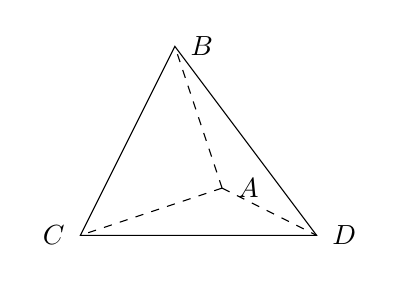
\begin{tikzpicture}[scale=.6]
    \coordinate[label=right:$A$](A)at(3,1);
    \coordinate[label=right:$B$](B)at(2,4);
    \coordinate[label=left:$C$](C)at(0,0);
    \coordinate[label=right:$D$](D)at(5,0);
    \draw(B)--(C)--(D)--cycle;
    \draw[dashed](A)--(B)(A)--(C)(A)--(D);
\end{tikzpicture}\end{wrapfigure}
则 $\triangle ABD, \triangle ACD$ 都是二奇一偶. 不妨设 $AC$ 的长也是奇数, 则 $CD$ 的长是偶数. 若 $AB$ 的长是奇数, 则 $BD,BC$ 的长都是偶数, 
这是三奇三偶的情形. 若 $AB$ 的长是偶数, 则 $BD,BC$ 的长都是奇数, 这是四奇二偶的情形. \par
\end{proof}
  
\subsection{直角海伦四面体}
\begin{definition}
   从一个顶点出发的三条棱两两垂直的四面体称为\emph{直角四面体}, 如果一个直角四面体也是海伦四面体, 就称之为\emph{直角海伦四面体}. 
\end{definition}

\begin{theorem}
    直角海伦四面体的体积是 6 的倍数. 
\end{theorem}
\begin{proof}
    设直角海伦四面体的三条直角边分别为$a,b,c$. 由于
    \begin{equation}\label{tiji32}
        V=\frac13\cdot\frac{bc}2\cdot a
    \end{equation}
    根据定理(\ref{mianji6}), $bc/2$被 6 整除, 所以$2|V$.\par
    根据推论(\ref{gougu3}), 不妨设$3|a$, 同理根据式(\ref{tiji32})可得$3|V$. 所以$6|V$. 
\end{proof}

\begin{theorem}
    本原直角海伦四面体的三条直角边$a,b,c$必定是一奇二偶. 
\end{theorem}
\begin{proof}
    首先, 因为是本原的, 所以$a,b,c$中必有一个奇数. 又直角海伦三角形必有一条直角边是偶数, 所以$a,b$中必有一个是偶数, $a,c$必有一个是偶数, $b,c$也必有一个是偶数. 所以$a,b,c$中一奇二偶. 
\end{proof}

\begin{theorem}
    直角海伦四面体存在, 等价于下述方程组有整数解
    \begin{align}\label{youjie}
    \begin{cases}
        &a^2+b^2=d^2\\
        &a^2+c^2=e^2\\
        &b^2+c^2=f^2\\
        &a^2b^2+a^2c^2+b^2c^2=S^2
    \end{cases}\end{align}
\end{theorem}
\begin{proof}
    设直角四面体的底面面积为$S$. 运用解析几何的知识不难得出, 底面上的高为
    \[h=\frac{abc}{\sqrt{a^2b^2+a^2c^2+b^2c^2}}\]
    由四面体的体积公式有
    \[V=\frac13S\frac{abc}{\sqrt{a^2b^2+a^2c^2+b^2c^2}}=\frac16abc\]
    所以
    \[S=\frac12\sqrt{a^2b^2+a^2c^2+b^2c^2}.\]
    若存在直角海伦四面体, 显然方程组(\ref{youjie})有解. 反之, 若方程组(\ref{youjie}), 则以$a,b,c$作为一条直角边的四面体是直角海伦四面体. 
\end{proof}

\subsection{直角海伦四面体与完美长方体的联系}
完美长方体存在, 等价于下述方程组有整数解
\begin{align*}
\begin{cases}
    &a^2+b^2=d^2\\
    &a^2+c^2=e^2\\
    &b^2+c^2=f^2\\
    &a^2+b^2+c^2=g^2
\end{cases}
\end{align*}
截止2007年10月, 还没有找到任何完美长方体, 亦未有人证明完美长方体不存在. 
\begin{theorem}
    如果存在直角海伦四面体, 则存在完美长方体.
\end{theorem}
\begin{proof}
    如果存在直角海伦四面体, 则方程组(\ref{youjie})有解, 从而方程组
    \begin{align*}\hspace{2.5em}\begin{cases}
        &a^2b^2+a^2c^2=d^2\\
        &a^2b^2+b^2c^2=e^2\\
        &a^2c^2+b^2c^2=f^2\\
        &a^2b^2+a^2c^2+b^2c^2=g^2
    \end{cases}\end{align*}
有解, 这蕴含存在完美长方体. 
\end{proof}

\subsection{等腰海伦四面体}
\begin{definition}
    三组对棱分别相等的四面体称为\emph{等腰四面体}, 如果一个等腰四面体也是海伦四面体, 就称之为\emph{等腰海伦四面体}. 
\end{definition}

设四面体的三组相对的对棱的长分别为$a,a',b,b',c,c'$, 其体积为$V$, 记
    \begin{align*}
        M_a &= (aa')^2(b^2+b'^2+c^2+c'^2-a^2-a'^2) \\
        M_b &= (bb')^2(a^2+a'^2+c^2+c'^2-b^2-b'^2)\\
        M_c &= (cc')^2(a^2+a'^2+b^2+b'^2-c^2-c'^2)\\
        N \ &= (abc)^2+(ab'c')^2+(a'bc')^2+(a'b'c)^2
    \end{align*}
则$V=\dfrac1{12}\sqrt{M_a+M_b+M_c-N}$.\upcite{yuzhi}\\[1pt]

特别地, 令$a'=a,b'=b,c'=c$可得三组对棱的长分别相等的四面体(这种四面体被称为等腰四面体)的体积为
    \begin{equation}\label{dengyaosimian}
         V=\frac{\sqrt2}{12}\sqrt{(a^2+b^2-c^2)(a^2+c^2-b^2)(b^2+c^2-a^2)} 
    \end{equation}

令$k^2=(a^2+b^2+c^2)/2$则
    \begin{equation*}\label{tijik}
        V=\dfrac12\sqrt{(k^2-a^2)(k^2-b^2)(k^2-c^2)}.
    \end{equation*}

\begin{theorem}
    等腰海伦四面体的四个面是全等的锐角海伦三角形. 
\end{theorem}
\begin{proof}
    这个定理实际上有三个命题, \circled1四个面都是海伦三角形; \circled2四个面都是锐角三角形; \circled3四个面是全等三角形. \circled1是显然的. 下面我们证明\circled2. 

如图, 设等腰海伦四面体的六条边长分别为$a,a,b,b,c,c$, 则它的四个面都是边长为$a,b,c$的三角形, 所以它们都是全等三角形. 

接下来只需证明这个边长为$a,b,c$的海伦三角形是锐角三角形. 反设$a,b,c$不是一 个锐角三角形, 则$a^2+b^2-c^2$, $a^2+c^2-b^2$, $b^2+c^2-a^2$必有一个在于等于零, 另外两个小于等于零, 这与式(\ref{dengyaosimian})产生矛盾, 所以等腰海伦四面体的四个面都锐角三角形. 
\end{proof}

\msection{致谢}
感谢王正攀老师对我的悉心指导。王老师是我大学的启蒙老师,大一的时候就传授给我一些思想,大四毕业之际又帮助我完成毕业论文,我发自内心地感谢他。同时也要谢谢我的母亲,在我写作的过程中鼓励我。

\begin{mybib}
\bibitem{daoxuan}朱道勋. 关于海伦三角形的边和面积的性质[J]. 数学通迅, 1994(09): 20-21
\bibitem{denggao}曾登高. 海伦数组的若干注记[J]. 中学数学, 1995年05期: 37-37
\bibitem{huangxi}黄曦. 本原海伦三角形的边的问题[J]. 沙洋师范高等专科学校学报, 2011(05): 44-45.%期刊类
\bibitem{keqin}冯克勤. 平方和[M]. 哈尔滨: 哈尔滨工业大学出版社, 2011: 1-5
\bibitem{cihe}闵嗣鹤, 严士健. 初等数论[M]. 北京: 高等教育出版社, 2003: 91-103 %书籍
\bibitem{kezhao}柯召, 孙琦. 谈谈不定方程[M]. 哈尔滨: 哈尔滨工业大学出版社, 2011: 18-23
\bibitem{carlson}Carlson, John R. (1970), Determination of Heronian Triangles(PDF), Fibonacci Quarterly 8: 499–506
\bibitem{oeis}Online Encyclopedia of Integer Sequences, OEIS A011943.
\bibitem{chengjun}程俊. 关于连续海伦三角形的研究[J]. 中学数学教学参考, 1991(12): 37-38
\bibitem{jianyi}沈建仪. 海伦三角形和海伦数[J]. 无锡市广播电视大学学报, 2008(2): 49-52
\bibitem{yaoyong}姚勇. 周长是面积 k 倍的海伦三角形[J]. 数学通迅, 1996(02): 29-29
\bibitem{bianxin}边欣, 李忠民. 有关本原海伦三角形的几个新的结论[J]. 数学通迅, 1995(10), 26-27
\bibitem{liuyi}刘毅, 杨杰飞. 周长与面积相等的海伦三角形[J]. 数学通迅, 1995(04): 15-16

\bibitem{huaming}苏化明. 等腰四面体的一些性质和主要不变量之间的关系[J]. 中学数学教学, 1983(01), 14-16
\bibitem{yuzhi}余志. 四面体的六棱求积公式[J]. 数学通迅, 2003(19): 31-31
\end{mybib}


\msection{附录}
\begin{table}[H]
\centering
\bicaption{表}{周长不超过 100 的海伦三角形}{Table}{Heronian triangle circumference less than 100 }
\begin{tabular}{lllllrrrrr}
\toprule
边长&边长&边长&周长&面积 &       边长&边长&边长&周长&面积\\
\midrule
3  & 4  & 5  & 12 & 6   &	5  & 5  & 6  & 16 & 12 \\
5  & 5  & 8  & 18 & 12  &	6  & 8  & 10 & 24 & 24 \\
5  & 12 & 13 & 30 & 30  &	4  & 13 & 15 & 32 & 24 \\
10 & 10 & 12 & 32 & 48  &	9  & 10 & 17 & 36 & 36 \\
9  & 12 & 15 & 36 & 54  &	10 & 10 & 16 & 36 & 48 \\
10 & 13 & 13 & 36 & 60  &	8  & 15 & 17 & 40 & 60 \\
7  & 15 & 20 & 42 & 42  &	13 & 14 & 15 & 42 & 84 \\
11 & 13 & 20 & 44 & 66  &	10 & 17 & 21 & 48 & 84 \\
12 & 16 & 20 & 48 & 96  &	15 & 15 & 18 & 48 & 108\\
13 & 13 & 24 & 50 & 60  &	16 & 17 & 17 & 50 & 120\\
3  & 25 & 26 & 54 & 36  &	12 & 17 & 25 & 54 & 90 \\
13 & 20 & 21 & 54 & 126 &	15 & 15 & 24 & 54 & 108\\
7  & 24 & 25 & 56 & 84  &	6  & 25 & 29 & 60 & 60 \\
10 & 24 & 26 & 60 & 120 &	15 & 20 & 25 & 60 & 150\\
5  & 29 & 30 & 64 & 72  &	8  & 26 & 30 & 64 & 96 \\
14 & 25 & 25 & 64 & 168 &	17 & 17 & 30 & 64 & 120\\
20 & 20 & 24 & 64 & 192 &	11 & 25 & 30 & 66 & 132\\
17 & 25 & 26 & 68 & 204 &	17 & 25 & 28 & 70 & 210\\
20 & 21 & 29 & 70 & 210 &	8  & 29 & 35 & 72 & 84 \\
18 & 20 & 34 & 72 & 144 &	18 & 24 & 30 & 72 & 216\\
20 & 20 & 32 & 72 & 192 &	20 & 26 & 26 & 72 & 240\\
19 & 20 & 37 & 76 & 114 &	15 & 26 & 37 & 78 & 156\\
13 & 30 & 37 & 80 & 180 &	16 & 25 & 39 & 80 & 120\\
16 & 30 & 34 & 80 & 240 &	25 & 25 & 30 & 80 & 300\\
10 & 35 & 39 & 84 & 168 &	12 & 35 & 37 & 84 & 210\\
14 & 30 & 40 & 84 & 168 &	15 & 28 & 41 & 84 & 126\\
15 & 34 & 35 & 84 & 252 &	17 & 28 & 39 & 84 & 210\\
21 & 28 & 35 & 84 & 294 &	26 & 28 & 30 & 84 & 336\\
22 & 26 & 40 & 88 & 264 &	9  & 40 & 41 & 90 & 180\\
13 & 37 & 40 & 90 & 240 &	15 & 36 & 39 & 90 & 270\\
25 & 25 & 40 & 90 & 300 &	25 & 29 & 36 & 90 & 360\\
12 & 39 & 45 & 96 & 216 &	15 & 37 & 44 & 96 & 264\\
20 & 34 & 42 & 96 & 336 &	24 & 32 & 40 & 96 & 384\\
30 & 30 & 36 & 96 & 432 &	13 & 40 & 45 & 98 & 252\\
17 & 40 & 41 & 98 & 336 &	24 & 37 & 37 & 98 & 420\\
25 & 25 & 48 & 98 & 168 &	25 & 34 & 39 & 98 & 420\\
29 & 29 & 40 & 98 & 420 &	17 & 39 & 44 & 100& 330\\
18 & 41 & 41 & 100 & 360&	26 & 26 & 48 & 100& 240\\
29 & 29 & 42 & 100 & 420&	32 & 34 & 34 & 100& 480\\
\bottomrule
\end{tabular}%\label{tab:addlabel}%
\end{table}%

\begin{table}[H]
\centering
\bicaption{表}{周长和面积相等的海伦三角形}{Table}{Heronian triangle Circumference is equal to area}
\begin{tabular}{lllll}
\toprule
边长&边长&边长&周长&面积 \\
\midrule
6 & 8  & 10 & 24 & 24 \\
5 & 12 & 13 & 30 & 30 \\
9 & 10 & 17 & 36 & 36 \\
7 & 15 & 20 & 42 & 42 \\
6 & 25 & 29 & 60 & 60 \\
\bottomrule
\end{tabular}%\label{tab:addlabel}%
\end{table}%

\begin{table}[H]
\centering
\bicaption{表}{腰长小于 100 的本原等腰海伦三角形}{Table}{Primitive Heronian isosceles triangles that Waist-length less than 100}
\begin{tabular}{lllrrr}
\toprule
    边长&边长&边长&边长&边长&边长\\
\midrule
    5  & 5  & 6   & 5  & 5  & 8 \\
    13 & 13 & 10  & 13 & 13 & 24 \\
    17 & 17 & 16  & 17 & 17 & 30 \\
    25 & 25 & 14  & 25 & 25 & 48 \\
    29 & 29 & 40  & 29 & 29 & 42 \\
    37 & 37 & 24  & 37 & 37 & 70 \\
    41 & 41 & 18  & 41 & 41 & 80 \\
    53 & 53 & 56  & 53 & 53 & 90 \\
    61 & 61 & 22  & 61 & 61 & 120 \\
    65 & 65 & 32  & 65 & 65 & 66 \\
    65 & 65 & 112 & 65 & 65 & 126 \\
    73 & 73 & 96  & 73 & 73 & 110 \\
    85 & 85 & 26  & 85 & 85 & 72 \\
    85 & 85 & 154 & 85 & 85 & 168 \\
    89 & 89 & 78  & 89 & 89 & 160 \\
    97 & 97 & 130 & 97 & 97 & 144 \\
\bottomrule
\end{tabular}%\label{tab:addlabel}%
\end{table}%


\begin{table}[H]
\centering
\bicaption{表}{前 20 个边长是连续整数的海伦三角形}{Table}{Top 20 Heronian triangle with consecutive integers side}
\begin{tabular}{lllll}
    \toprule
    边长&边长&边长&周长&面积\\
    \midrule
    3           & 4           & 5           & 12           & 6\\
    13          & 14          & 15          & 42           & 84\\
    51          & 52          & 53          & 156          & 1170\\
    193         & 194         & 195         & 582          & 16296\\
    723         & 724         & 725         & 2172         & 226974\\
    2701        & 2702        & 2703        & 8106         & 3161340\\
    10083       & 10084       & 10085       & 30252        & 44031786\\
    37633       & 37634       & 37635       & 112902       & 613283664\\
    140451      & 140452      & 140453      & 421356       & 8541939510\\
    524173      & 524174      & 524175      & 1572522      & 118973869476\\
    1956243     & 1956244     & 1956245     & 5868732      & 1657092233154\\
    7300801     & 7300802     & 7300803     & 21902406     & 23080317394680\\
    27246963    & 27246964    & 27246965    & 81740892     & 321467351292366\\
    101687053   & 101687054   & 101687055   & 305061162    & 4477462600698444\\
    379501251   & 379501252   & 379501253   & 1138503756   & 62363009058485850\\
    1416317953  & 1416317954  & 1416317955  & 4248953862   & 868604664218103456\\
    5285770563  & 5285770564  & 5285770565  & 15857311692  & 12098102289994962534\\
    19726764301 & 19726764302 & 19726764303 & 59180292906  & 168504827395711372020\\
    73621286643 & 73621286644 & 73621286645 & 220863859932 & 2346969481249964245746\\
\bottomrule
\end{tabular}%\label{tab:addlabel}%
\end{table}%


\end{document} 


